\documentclass{beamer}

\title{TDD Kata}
\author{Jun Chen}
%\date{June 15, 2005}

%\usepackage{beamerthemeBerlin}

\usetheme{Luebeck}
\usecolortheme{beaver}

%\usetheme{Antibes}
%\usecolortheme{lily} 

\begin{document}
%\maketitle

\begin{frame}
\titlepage
\end{frame}

% \begin{frame}
%  \frametitle{Outline}
%   \tableofcontents[part=1, pausesections]
% \end{frame}

\begin{frame}
 \frametitle{TDD Cycle: Red-Green-Refactor}

 \begin{columns}

 %\column{1.5in}
 \column{.45\textwidth}
 %\begin{center}
 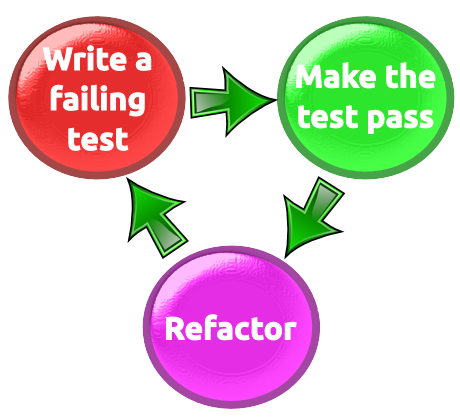
\includegraphics[height=2.0in]{TDD-cycle}
 %\end{center}

 %\column{1.5in}
 \column{.55\textwidth}
 \begin{itemize}
  \item \small {Write a test ("red")}
  \item \small {Get the test to pass ("green")}
  \item \small {Optimize the design ("refactor")}
 \end{itemize}
 \end{columns}
 \pause
 Each test should represent the smallest meaningful increment you can think of.
\end{frame}

\begin{frame}
 \frametitle{Three Rules of TDD}
 \pause
 \begin{enumerate}
  \item Write \alert{NO} production code except to pass a failing test.
  \pause
  \item Write only \alert{enough} of a test to demonstrate a failure.
  \pause
  \item Write only \alert{enough} production code to pass the test.
 \end{enumerate}
\end{frame}

\begin{frame}
 \frametitle{Scoring Bowling}
  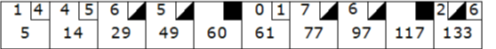
\includegraphics[height=0.2in]{Bowling} \\
The game consists of 10 frames as shown above.  In each frame the player has
two opportunities to knock down 10 pins.  The score for the frame is the total
number of pins knocked down, plus bonuses for strikes and spares.\\
 \begin{enumerate}
 \item \alert{A spare} is when the player knocks down all 10 pins in two tries.  The bonus for
that frame is the number of pins knocked down by the next roll.  So in frame 3
above, the score is 10 (the total number knocked down) plus a bonus of 5 (the
number of pins knocked down on the next roll.)\\

 \item \alert{A strike} is when the player knocks down all 10 pins on his first try.  The bonus
for that frame is the value of the next two balls rolled.\\

 \item In the tenth frame a player who rolls a spare or strike is allowed to roll the extra
balls to complete the frame.  However no more than three balls can be rolled in
tenth frame.
 \end{enumerate}

\end{frame}

\begin{frame}
 \frametitle{Requirement}
Write a class named “Game” that has two methods
  \begin{enumerate}
  \item roll(pins : int) is called each time the player rolls a ball.  The argument is the number of pins knocked down.
  \item score() : int is called only at the very end of the game.  It returns the total score for that game.
  \end{enumerate}
\end{frame}

\end{document}
